\chapter{Cottontail DB}
\epiquote{All the world will be your enemy, Prince with a Thousand Enemies, and whenever they catch you, they will kill you. But first they must catch you, digger, listener, runner, prince with the swift warning. Be cunning and full of tricks and your people shall never be destroyed.}{Richard Adams, 1972}

\label{chapter:cottontaildb}

\cottontail{}~\cite{Gasser:2020Cottontail} is our reference implementation for the query, cost and index maintenance models described in \Cref{chapter:system_model}. Starting out as a drop-in replacement for ADAMpro \cite{Giangreco:2016Adam}, it has grown to be a full fledged \acrshort{dbms} with support for classical Boolean, fulltext\footnote{Powered by Apache Lucene, See https://lucene.apache.org/} as well as proximity based search used in multimedia retrieval and analytics applications in the \vitrivr{} \cite{Rossetto:2016Vitrivr,Gasser:2019Multimodal} context. All three aspects are combined in a unified query and execution model and many explicit and implicit decisions, which are described in this chapter, went into its conception and design.

\cottontail{} is written in Kotlin\footnote{See: https://kotlinlang.org/} and runs on the \acrfull{jvm}. \cottontail{}'s source code can be downloaded from GitHub\footnote{See: https://github.com/vitrivr/cottontaildb}. It is freely available under a permissive open source license and can be used as standalone application, Docker container or in an embedded mode.

\section{Data Model and Nomenclature} 

\cottontail{} uses a data model very similar to that of other relational \acrshort{dbms}': All data is organized into \emph{entities} -- which correspond to tables or relations. Every entity consists of individual, strongly typed \emph{columns}. The different data types currently supported are listed in \Cref{table:cottontail_types}. Columns can hold values of the declared type or \texttt{NULL} to indicate the absence of information, if the column has been declared as being nullable. To support the features used in multimedia retrieval applications, vector types are first-class members the type system.

\begin{table}[bt]
    \caption{Data types supported by \cottontail{}. Types in the numeric, vector and complex class allow for domain specific arithmetics.}
    \label{table:cottontail_types}

    \begin{tabular}{| l || c | c | c | c | l |}
        \hline
        \textbf{Name} & \textbf{Scalar} & \textbf{Numeric} & \textbf{Vector} & \textbf{Complex} & \textbf{JDBC / SQL}\\ 
        \hline
        \hline
        String & \cmark & \xmark & \xmark & \xmark & \texttt{VARCHAR} \\ 
        \hline
        ByteString & \cmark & \xmark & \xmark & \xmark & \texttt{BLOB} \\ 
        \hline
        Date & \cmark & \xmark & \xmark & \xmark & \texttt{TIMESTAMP}\\
        \hline 
        Boolean & \cmark & \cmark & \xmark & \xmark & \texttt{BOOLEAN} \\ 
        \hline
        Byte & \cmark & \cmark & \xmark & \xmark & \texttt{TINYINT} \\ 
        \hline
        Short & \cmark & \cmark & \xmark & \xmark & \texttt{SMALLINT} \\ 
        \hline
        Int & \cmark & \cmark & \xmark & \xmark & \texttt{INT}\\ 
        \hline
        Long & \cmark & \cmark & \xmark & \xmark & \texttt{BIGINT}\\ 
        \hline
        Float & \cmark & \cmark & \xmark & \xmark & \texttt{REAL}\\ 
        \hline
        Double & \cmark & \cmark & \xmark & \xmark & \texttt{DOUBLE}\\ 
        \hline
        Complex 32 & \cmark & \xmark & \xmark & \cmark & - \\ 
        \hline
        Complex 64 & \cmark & \xmark & \xmark & \cmark & - \\ 
        \hline
        Boolean Vector & \xmark & \xmark & \cmark & \xmark & \texttt{ARRAY[BOOLEAN](1, d)} \\ 
        \hline
        Integer Vector & \xmark & \xmark & \cmark & \xmark & \texttt{ARRAY[INT](1, d)} \\ 
        \hline
        Long Vector & \xmark & \xmark & \cmark & \xmark & \texttt{ARRAY[BIGINT](1, d)}\\ 
        \hline
        Float Vector & \xmark & \xmark & \cmark & \xmark & \texttt{ARRAY[REAL](1, d)}\\ 
        \hline
        Double Vector & \xmark & \xmark & \cmark & \xmark & \texttt{ARRAY[DOUBLE](1, d)}\\ 
        \hline
        Complex32 Vector & \xmark & \xmark & \cmark & \cmark & - \\ 
        \hline
        Complex32 Vector & \xmark & \xmark & \cmark & \cmark & - \\ 
        \hline
    \end{tabular}
\end{table}

An entity can host multiple \emph{records}, which correspond to tuples in the relation. Since \cottontail{} is a column store, records are only logical constructs in memory and do not reflect the physical data representation on disk. Consequently, records are assembled on-the-fly as queries are being executed. Similarily to columns, every record is also strongly typed, wherein a record is a tuple type of its strongly typed elements. Internally, every record is uniquely identified by a \emph{tuple identifier} (\texttt{TID}), which is a \texttt{long} value that can be used to address the record within an entity or an (in-memory) \emph{recordset}. This \texttt{TID} is not exposed to the outside because it remains at the discretion of the storage and execution engine to generate, assign, change and (re-)use them as data gets (re-)organised.

Furthermore, \cottontail{} allows for multiple entities to be grouped into \emph{schemata}, which currently serves an organisational purpose only. Every entity can also host one or multiple secondary \emph{indexes} that index a single or multiple \emph{columns} for more efficient data access. In addition to indexes for Boolean and fulltext search, \cottontail{} also hosts different types of high-dimensional index structures used for proximity based queries, for example, \acrshort{pq} \cite{Jegou:2010Product}, \acrshort{vaf} \cite{Weber:1998Va} and \acrshort{lsh}-based \cite{Indyk1998:Approximate} indexes.

To address database objects, \cottontail{} uses a hierarchical namespace, i.e., every schema, entity, column and index must be uniquely named by a \emph{fully qualified name}. All the information about the database objects -- including all column and index statistics  -- is tracked in an internal \emph{catalogue}, which is backed by the main storage engine.


\section{Architecture} 

The main components of \cottontail{} are depicted in \Cref{figure:cottontail_architecture}. We use the path a query takes within the system, as indicated by the directed arrows, to illustrate the components involved in its implementation.

At a high level, every query must undergo \emph{parsing}, \emph{binding}, \emph{planning} and \emph{execution} in that order, even though, planning may be skipped for certain types of queries (e.g. \acrshort{ddl} statements) or upon request. Starting with the binding step, all the information required for query processing is accumulated in a \emph{query context} object, which is passed between the steps. In the following sections, we will describe the aforementioned steps in reverse order, since important concepts can be introduced more naturally that way.

\begin{figure}[bt]
    \centering
    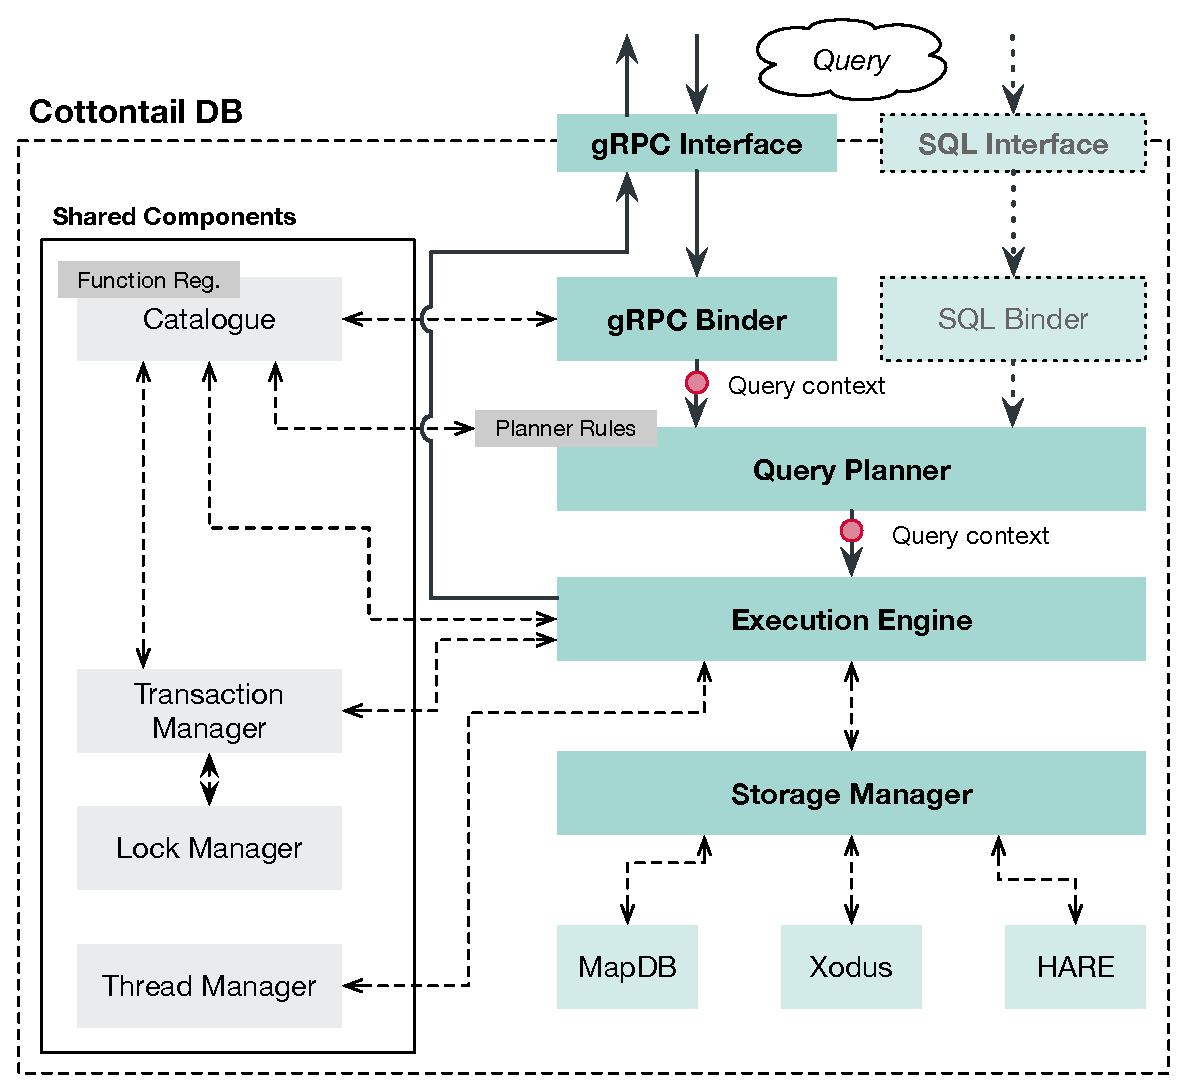
\includegraphics[width=\textwidth]{figures/architecture.eps}
    \caption{Architecture diagram of \cottontail{}'s main components. The directed arrows indicate the path a query takes within the system (dashed for a potential SQL interface). The dashed, double arrows indicate interactions between components.}
    \label{figure:cottontail_architecture}
\end{figure}


\subsection{Query Implementation and Execution}

\cottontail{} implements an \emph{iterator model} for query execution. This means that an implemented query is a pipeline of operators, wherein each operator processes single records it receives from its upstream (input) operator(s) and passes single records to the next operator in the pipeline. Most operators have a direct correspondence to the relational operators (\Cref{chapter:theory_databases}) and extensions (\Cref{chapter:system_model}) introduced thus far. However, not all operators behave exactly as required by the model due to implementation details. For example, the \texttt{FETCH} operation corresponds to a variant of the projection $\projection$ but instead of projecting onto a subset of the incoming attributes, it extends them, by looking up values in the database, i.e. logically (logically, \texttt{FETCH} corresponds to the operation $\symop(\relation) \Join_{\mathtt{TID}} \projection_{\attribute_{+}}(\relation)$ for the additional attribute $\attribute_{+} \in \schema(\relation)$, wherein the join acts on the tuple identifier). Such an operation can be beneficial since \cottontail{} allows for access to individual columns and thus it can reduce the cost of IO to defer access to certain columns.

Conceptually, \cottontail{} distinguishes between \emph{Nullary}, \emph{Unary}, \emph{Binary} and \emph{N-Ary} operators, which differ in the number of inputs they can accept (0, 1, 2 or N). Furthermore, some operators require materialization of intermediate resultsets and therefore act as pipeline breakers since they must collect all inbound records before they can start handing them down (e.g., sort operator). The most important types of operators implemented by \cottontail{} along with their correspondence to the relational operators are listed in \Cref{table:cottontail_operators}. Every operator is implemented in Kotlin and pre-compiled to byte code.

\begin{table}
    \caption{Main types of physical operators implemented by \cottontail{} alongside with their arity, their correspondence to relational operators and whether or not they require materialization.}
    \label{table:cottontail_operators}

    \begin{tabular}{| l || c | p{30mm}  | c | p{70mm} |}
        \hline
        \textbf{Type} & \textbf{Arty} & \textbf{Rel. Op.} & \textbf{Mat.} & \textbf{Description} \\ 
        \hline
        \hline
        \texttt{SCAN} & 0 & $\projection_{P}(\relation)$ \newline $\rho_{\attribute_{\mathtt{A} \rightarrow \attribute_\mathtt{B}}}(\projection_{P}(\relation))$ & & Act as a data source. Scans an \emph{entity} and interacts directly with the storage manager. \\ 
        \hline
        \texttt{INDEX} & 0 & $\selection_{S}(\relation)$ \newline $\projection_{\symdist}(\relation)$ \newline $\order_{\attribute_{d\updownarrow}}(\projection_{\symdist}(\relation))$ \newline $\limit_k(\order_{\attribute_{d\updownarrow}}(\projection_{\symdist}(\relation))) $ & & Acts as data source. Scans an \emph{index} and interacts directly with the storage manager. Can be any type of operator sequence outlined in \Cref{section:dfc_and_indexes} \\ 
        \hline
        \texttt{FETCH} & 1 & $\Join_{\mathtt{TID}}(\cdot, \projection_{\attribute_{+}}(\relation))$ & & Extends every incoming record by fetching values for one or multiple columns and appending them to the record. This is a specialised projection that extends the columns present in the outgoing relation. \\
        \hline 
        \texttt{FUNCTION} & 1 & $\Join_{\mathtt{TID}}(\cdot, \projection_{f(\cdot)}(\relation))$ & & Extends every incoming record by evaluating a specific function and appending the result as a new column to the record. This is a specialised projection that extends the columns present in the outgoing relation. \\ 
        \hline
        \texttt{FILTER} & 1 & $\selection_{S}(\cdot)$ & & Filter incoming records by evaluating a given predicate. Records that don't match the predicate are not handed down the pipeline. \\ 
        \hline
        \texttt{SORT} & 1 & $\order_{O}(\cdot)$ & \cmark & Sort the incoming records based on the specified columns in the specified direction. \\ 
        \hline
        \texttt{LIMIT} & 1 & $\limit_k(\cdot)$ & &  Skip and drop incoming records according to specification and thus limit the number of out-bound records to a specified number \\ 
        \hline
        \texttt{PROJECT} & 1 & $\projection_{P}(\cdot)$ \newline $\rho_{\attribute_\mathtt{A} \rightarrow \attribute_\mathtt{B}}$ & & A terminal operator that actively removes and/or renames columns in the incoming records. This is sometimes necessary because columns that are fetched for processing may not be desired in the final result. \\ 
        \hline
        \texttt{MERGE} & N & - & & An operator that merges tuples from incoming strands of query execution in an arbitrary order (union semantics). Used for intra-query parallelism. \\ 
        \hline
        \hline
    \end{tabular}  
\end{table}

\subsubsection{Execution Model}

Operators in \cottontail{} are implemented as \emph{coroutines}, i.e., every operator is a suspendable function that yields to the next operator in the pipeline upon emission of a value. Each operator collects a single record from its input operator(s), performs processing and forwards the resulting record by calling \texttt{emit()}, thus yielding to the next operator in the pipeline. Source operators usually iterate some data collection through a cursor and thus only \texttt{emit()} values, whereas sink operators \texttt{collect()} values without emiting anything (practically, the collected values are usually sent to the client that issued the query). Pipeline breaking operators are required to \texttt{collect()} all inbound values before they can start to \texttt{emit()}, i.e., they materialize a recordset. The suspension and continuation of operator calls is orchestrated by Kotlin \emph{Flows}, which are part of its coroutines framework. An example of a naive operator pipeline is provided in \Cref{figure:cottontail_execution_model_simple}. 

\begin{figure}[bt]
    \centering
    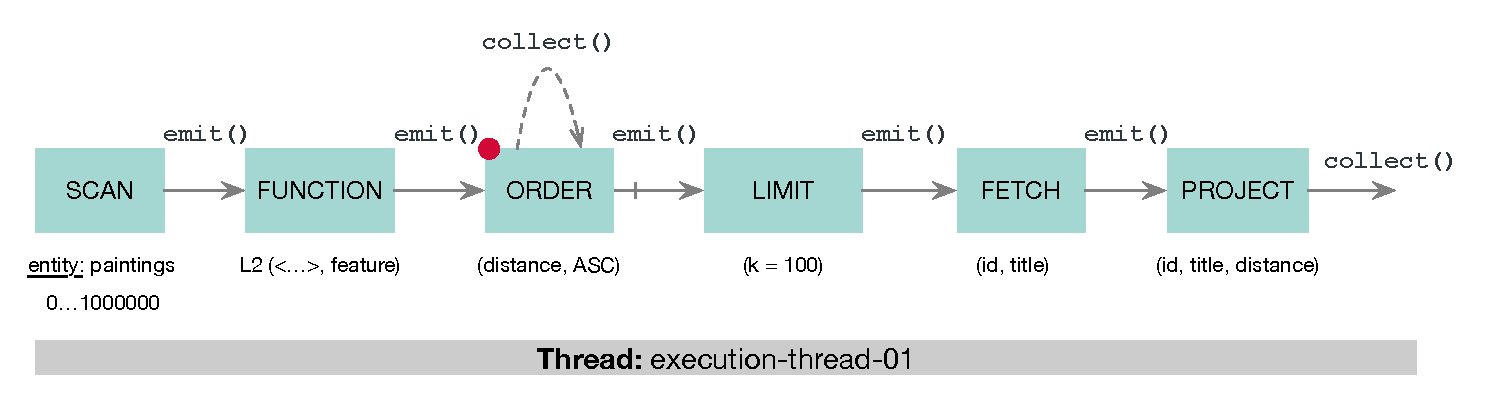
\includegraphics[width=0.9\textwidth]{figures/execution-model-simple}
    \caption{Operator pipeline for a proximity based query that scans the entity \emph{paintings}, calulates the L2 distance between a \emph{feature} column and a query, orders by the obtained distance and limits the number of outputs (\acrshort{knn}). Pipeline breaking operators are indicated by the red dot.}
    \label{figure:cottontail_execution_model_simple}
\end{figure}

Inter-query parallelism is achieved by collecting different operator pipelines on different threads. The assignment of operator pipeline to thread is delegated to a \emph{dispatcher}, which has a defined thread pool at its disposal and is also part of Kotlin's coroutines framework. Transaction isolation is guaranteed at all time by the \emph{transaction manager} and is achieved through \emph{snapshot isolation}. In addition, this execution model also allows for intra-query parallelism, which is used for queries that incur a high CPU cost. Intra-query parallelism is realised in a \emph{data parallel} fashion by partitioning on the input. The decision whether or not to allow for parallelism is made upon implementation of a query -- i.e., the last step after the final plan has been selected -- since it requires structural changes to the operator pipeline. The degree of parallelism depends on the expected CPU cost of the plan and the available CPUs on the machine \cottontail{} is running on.

To prepare for intra-query parallelism, part of the operator pipeline is partitioned wherein every partition operates on a fraction of the input data. Whether partitioning is possible at a given point in the pipeline depends on whether the operator itself as well as all upstream operators allow for partitioning, which is queried upon implementation of the plan. An additional concurrency aware \texttt{MERGE} operator is introduced after such a partitioning point, which synchronizes and merges all the incoming strands using a \acrshort{fifo} scheme. Since \texttt{MERGE} operators do not retain ordering, the sort operations must take place afterwards. An example for this is given in \Cref{figure:cottontail_execution_model_parallel}. In practic, the three steps are combined into a single operator.

\begin{figure}[bt]
    \centering
    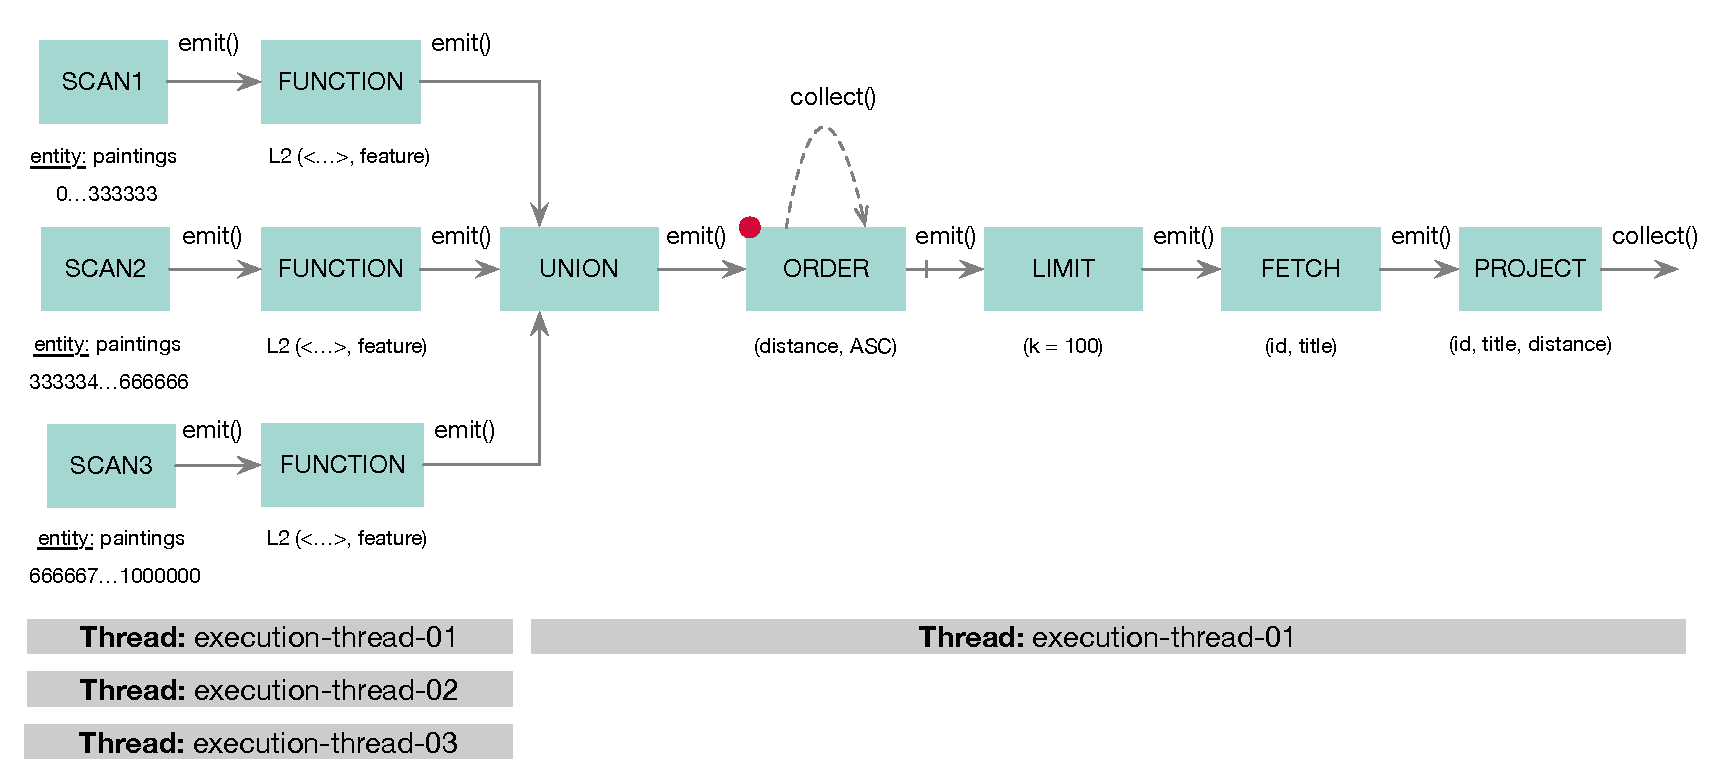
\includegraphics[width=0.9\textwidth]{figures/execution-model-parallel}
    \caption{Operator pipeline that performs \acrshort{knn} on the entity \emph{paintings}. The \emph{scan} and distance \emph{function} steps are partitioned and merged before order, limit and projection is applied, which allows for parallel execution.}
    \label{figure:cottontail_execution_model_parallel}
\end{figure}

With an operator pipeline prepared in this fashion, it again remains up to the dispatcher to allocate parts of the pipeline to concrete threads. \cottontail{} only declares how allocation should take place by chosing the appropriate type of dispatcher. Scheduling then depends on available hardware and system load. Consequently, the number of partitions is merely an upper bound on parallelism without guarantee, that every strand will be processed in its own thread. 

\subsection{Query Planner}
\label{section:cottontail_query_planner}

The goal of \emph{query planning} is to find a cost-optimal execution plan for a query given any \emph{policy} valid for the current query context and \cottontail{}'s cost model outlined in \Cref{section:cost_model}. The input into the query planner is a logical representation of the operators that should be executed as part of the operator pipeline, which we call the \emph{canonical operator node tree}. It results directly from the \emph{query binding} stage.

Query planning in \cottontail{} then takes place in three steps: First, and optionally, the canonical operator node tree is compared to the \emph{plan cache}. If the cache contains a hit for that tree, the already optimised plan in the cache can be re-used and all the subsequent steps can be skipped. Second, if there is no hit in the cache or the cache is bypassed, the canonical operator node tree undergoes \emph{optimisation}. The optimisation step generates different versions of the input plan by applying optimisation rules that act on and manipulate the tree to generate new, equivalent plans. Finally, once optimisation has concluded, the plan that minimises the expected cost is selected and implemented.

\subsubsection{Optimisation Algorithm}

The query planner used by \cottontail{} is rather naive and can be categorized as a rule-based query planner. It is losely inspired by the Cascades Framework that was built as part of the Volcano project~\cite{Graefe:1993Volcano}. The planner generates new plans by enumerating and applying a set of rules to the input plan(s) in a recursive fashion. These rules are transformations that recognize patterns in the structure of the operator node tree and try to re-arange and/or replace nodes in the tree to generate a more optimal but equivalent version of the plan.

The optimisation follows the same, basic algorithm: The available list of rules is enumerated and every rule is applied to every node starting from the base of the tree. The application of rules takes place recursively, i.e., every node propagates a rule up the tree to its inputs. At every node, the rule first checks if it can be applied to the current node. This check usually incurs little cost and simply considers the type of node and other, available properties. If the check is successful, the actual application of the rule follows. This application may or may not yield a new version of the query plan, depending on more complex and more costly factors, such as the availability of an index, which requires a catalogue lookup. If a new plan results from the application of a rule, that new query plan is stored in a \emph{memoization table} for future reference. 

Every planning stage involves a defined number of passes, and the sum of all plans generated by one pass act as the input for the next. All the intermediate plans are therefore run through the same algorithm and all the rules are applied again. Consequently, the search space grows exponentially with the complexity of the input plan, the number of rules to apply and the number of passes. To address this issue, \cottontail{}'s query planner employs certain heuristics to keep the search space manageable:

\begin{itemize}
    \item Very large, complex plans (e.g., stemming from sub-selects) are broken into groups and every group is optimised and treated as an isolated plan. The assumption being that the combination of smaller, near-optimal plans must be close to optimal as well.
    \item The planning of every group is done in two stages -- a \emph{logical} and \emph{physical} stage -- with distinct and disjoint sets of rules. The results of the logical stage act as an input for the physical stage.
    \item Logical and physical query plans are uniquely identified by a hash. Memoization in combination with the aforementioned hash is used to track trees that have already been optimised and skip them.
    \item Physical execution plans generated in the second stage are actively pruned by the planner between the different passes based on the cost estimate.
\end{itemize}

Between the logical and the physical planning, there is a step that maps every logical operator node to its naive, physical counterpart. The number of passes per stage and active pruning of plans during the physical phase are used to steer the high-level behaviour of the query planner. During the logical phase, the goal is to generate as many, equivalent, logical query representations as possible to have a corpus of plans to optimize on (expansion phase). In contrast, during the physical phase, the planner tries to limit the number of intermediate plans to prevent the search space from exploding.

Once a collection of potential plans has been generated for each group, the query planer enumerates the (sub-)plans per group, determines the expected cost and selects the (sub-)plan that minimises it. It then reconstructs the full plan from the selected (sub-)plans, which is then implemented and executed. Furthermore, the mapping of the input plan to the resulting output plan is written to the plan cache.

\subsubsection{Plan Caching}

The plan cache is an optimisation mechanism that amortises the cost of the potentially expensive query planning if a certain type of query is encountered multiple times. At its core, the cache maps the hash code of every incoming canonical operator tree to the resulting, optimised physical plan. If the same query is encountered again, that plan can be looked-up and re-used directly, hence, avoiding another round of planning. Currently, there are certain limitations to the plan cache mechanism in \cottontail{}, which is why it is disabled by default. Firstly, the actual execution performance of a plan is not being evaluated against the cost model, i.e., the level of optimality of an execution plan is not assessed. And secondly, there is no mechanism that invalidates cached entries as changes to the data occur. 

\subsubsection{Logical Optimisation}

The logical optimisation step acts on structural properties of the operator node tree and aims at expanding the list of query plans in a way that increases the likelihood of finding the optimal plan during the physical phase. It basically leverages the algebraic properties of the operators involved, e.g., the ability to decompose a  \texttt{FILTER} operator evaluating a conjunction into two consecutive \texttt{FILTER} operators -- one for each side. This is illustrated in the example given in \Cref{figure:cottontail_logical_rule_conjunction}. The applicaton of this rule can be seen as a preparation for the physical optimisation phase, where specific predicates may be satisifed by a secondary index.

\begin{figure}[bt]
    \centering
    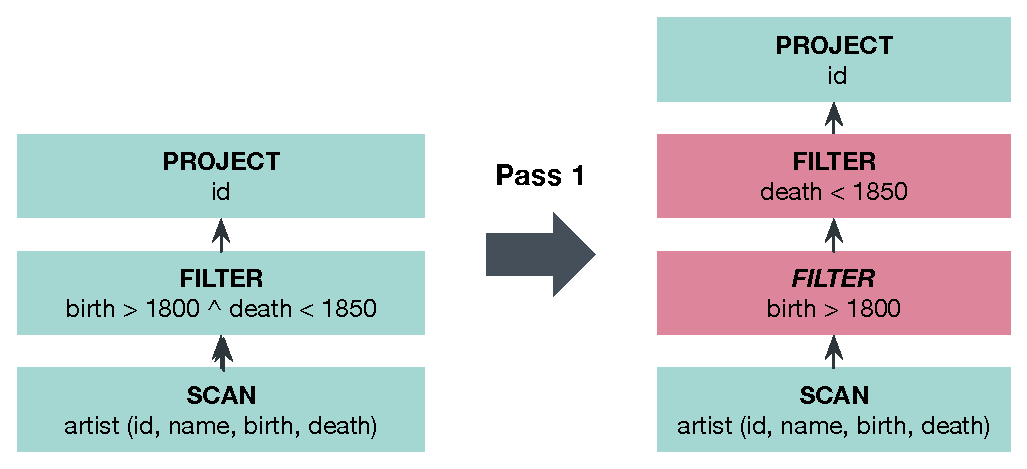
\includegraphics[width=0.9\textwidth]{figures/logical-rule-conjunction}
    \caption{Decomposition of conjunctive predicates. The filter on the column \texttt{death} may be pushed down at a later stage during physical optimisation, if an index were to be available.}
    \label{figure:cottontail_logical_rule_conjunction}
\end{figure}

\subsubsection{Physical Optimisation}

The physical optimisation step tries different implementations of operators to arrive at a more cost-effective plan. While structural changes to the operator tree may be possible, the focus lies on implementation aspects.  At a high level, we distinguish between the following types of rules:

\begin{description}
    \item[Index Replacement Rules] try to replace \texttt{FILTER} predicates or \texttt{FUNCTION} invocations with an  \texttt{INDEX} operation. For example, an entity \texttt{SCAN} followed by a \texttt{FILTER} can be replaced by a more efficient scan of a $B^{+}$-tree index followed by a \texttt{FETCH} operation or proximity based operations can be delegated to an available, high-dimensional index using the classes of index replacements listed in Definitions \ref{definition:dfc_index_class_1}, \ref{definition:dfc_index_class_2} and \ref{definition:dfc_index_class_3}.
 
    \item[Deferral Rules] try to defer the evaluation of functions and/or the fetching of columns to later stages of the query plan, which can be beneficial if a \texttt{LIMIT} or a \texttt{FILTER} leads to a reduction of the output cardinality. An example is given in \Cref{figure:cottontail_physical_rule_fetch}. This can significantly reduce IO. These rules also make sure, that only columns that are actually accesed are read from disk.

    \item[Summarization Rules]try to merge operations to arrive at a more efficient execution. For example, a \texttt{SORT} operation followed by a  \texttt{LIMIT} operation can be replaced by a single, \emph{limiting heap sort} operation, which applies sorting and limiting in a single step. Combining these two operations and the use of the heap-sort algorithm allows for more effective sorting in terms of CPU and memory cost, as compared to naively sorting all records first and then limiting to the top $k$ records thereafter.
    
    \item[Implementation Rules] simply replace different implementations of a operation one-to-one, e.g., hash-join vs. nested-loop join for a theoretical JOIN operation or a scalar version of a \texttt{FUNCTION} invocation by a vectorised version that uses \acrshort{simd} instructions.
\end{description}


\begin{figure}[bt]
    \centering
    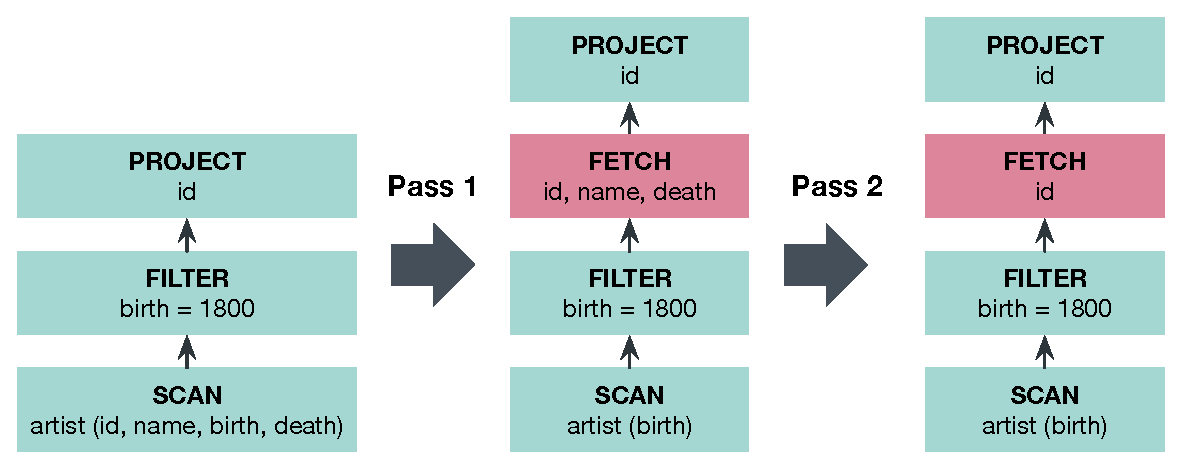
\includegraphics[width=0.9\textwidth]{figures/physical-rule-fetch}
    \caption{Illustration of deferring \texttt{FETCH} operations. Over multiple passes, the \texttt{FETCH} of the columns \texttt{id}, \texttt{name} and \texttt{death} is pushed up until after the \texttt{FILTER} has been applied. Columns \texttt{name} and \texttt{death} are eventually eliminated because they are not required.}
    \label{figure:cottontail_physical_rule_fetch}
\end{figure}

After each pass in the physical optimisation step, the list of resulting plans is pruned to the $n$ best performing plans before handing them to the next pass. By this, we limit the size of the search space that is being explored. Once all passes have concluded, the best plan in terms of cost is selected and implemented. We directly apply the cost model introduced and described in \Cref{chapter:system_model}.

\subsection{Query Parsing and Binding}
\cottontail{} uses a \emph{gRPC}\footnote{See: https://grpc.io/} based query language that allows for interaction with other systems. Hence, all queries are expressed as \emph{Protocol Buffer}\footnote{See: https://developers.google.com/protocol-buffers/} messages. These interactions include data definition, data management, transaction management and the formulation of queries. Internally, the gRPC endpoint is a collection of four services for handling \acrshort{ddl}, \acrshort{dml}, \acrshort{dql} and transaction management messages. The parsing of incoming messages, the mapping of messages to the correct service and endpoint and low-level handling of communication with clients is delegated to the gRPC Kotlin library. 

The reason for the choice of gRPC is threefold: Firstly, \cottontail{}'s predecessor -- ADAMpro~\cite{Giangreco:2016Adam} -- already used and introduced gRPC into the \emph{vitrivr} ecosystem. Consequently, building on this work greatly simplified the task of integrating \cottontail{}. Secondly, gRPC -- being a platform independent remote procedure call framework -- introduces out-of-the-box support for a large range of programming environments.\footnote{Furthermore, there are specialized client libraries for Java, Kotlin and Python} And finally, the gRPC Kotlin library greatly simplified the task of structuring query endpoints, parsing incoming query messages and handling the query responses.

Even though \cottontail{} uses gRPC, it can be seen as compatible with the SQL standard insofar as it supports a specific feature. This was demonstrated by be the successful integration of \cottontail{} as a storage engine for \emph{Polypheny-DB} \cite{Vogt:2018Polypheny,Vogt:2020Polypheny}. Consequently, it would be possible to add additional endpoints that can accept, for example, \acrshort{sql} queries. However, for complete SQL compliance, one would have to add language features that are currently not supported by \cottontail{} (e.g., JOINS). Furthermore, handling the technical details of parsing the incoming query and communication with the client must be handled as well, which would lead to the implementation of many different standards such as \acrshort{jdbc} or \acrshort{odbc}.

Irrespective of its source, any incoming query message undergoes a \emph{binding} step in \cottontail{}. Query binding includes three aspects:

\begin{enumerate}
    \item Names that reference database objects such as entities, columns and indexes are resolved using \cottontail{}'s catalogue and replaced by concrete pointers to the respective object.
    \item Literal values, function calls and column references, e.g., in predicates, are extracted and replaced by \emph{bindings} and attached to a \emph{binding context}.
    \item The parsed message is converted into a \emph{canonical operator node tree} that logically represents the query.
\end{enumerate}

The result of the parsing and binding step is the canonical operator node tree, which acts as a logical and unoptimised query representation.  Every node in the tree represents an operator that acts on a \emph{record} or \emph{tuple} and that must be executed in order to generate the result specified by the query. The conversion of a message to a tree is performed in a naive manner and only syntactic checks and optimisation are performed at this stage (e.g., type checks, removal of trivial predicates such as ''$1 = 1$``).

\subsubsection{Binding Context}
The binding context is a data structure that is member of the query context and a very important piece of functionality for query planning and execution. At their core, bindings are proxies for values used in a query. \cottontail{} distinguishes between \emph{literal}, \emph{column} and \emph{function} bindings. At any point during query execution, the binding context holds the current values for all the bindings associated with it, so that these can be accessed as the query is being evaluated.

The layer of indirection introduced by bindings enables many of \cottontail{}'s functionalities, e.g., in the evaluation of complex expressions for predicates or functions. Most importantly, however, it allows for re-use of query plans, as bindings can be simply rebound to another binding context. Plan re-use then simply comes down to copying a plan with all its bindings and assigning it a new binding context afterwards. 

With regards to intra-query parallelism, it is important to note that binding contexts are not thread-safe, which is why they are copied upon partitioning of a query plan. Consequently, every branch of an operator tree acts on its own child of the same, root binding context.

\subsection{Functions and Function Generators}

In compliance with the model proposed in \cref{chapter:system_model}, \cottontail{} implements a \emph{function registry}, which is part of the catalogue and can be used to obtain function implementations during query binding and planning. The function registry comprises of three components that are types of classes: The \texttt{FunctionRegistry} itself, \texttt{FunctionGenerator}s and \texttt{Function}s.

The registry is a singleton object that is kept in memory for an instance of \cottontail{}. It provides the interface to register function generators and resolve function implementations given a \emph{closed signature}. Function resolution then is facilitated by the \texttt{FunctionGenerator}, which are again singleton objects per type of \texttt{Function} -- e.g., Euclidean distance or scalar multiplication -- and act as factories for concrete \texttt{Function} implementations. A \texttt{FunctionGenerator} is always associated with an \texttt{OpenSignature}, which comprises of a \texttt{Function}'s name and potentially \emph{open} arguments, which only specify the class (e.g., number, vector) but not the concrete type (e.g., float number, double vector) of arguments. It is then up to the \texttt{FunctionGenerator} to return an implementation based on a \texttt{ClosedSignature}, if such an implementation exists.

Given this facility, function resolution takes place in two steps: First, a \texttt{ClosedSignature} is converted to an \texttt{OpenSignature} to lookup the responsible \texttt{FunctionGenerator} in a map. That generator then produces the concrete implementation, based on the \texttt{ClosedSignature}. This two-step process allows for easy extension, since adding new functions comes down to adding a generator and the type-specific implementations. Furthermore, the mechanism could be adapted to generate code at runtime, which \cottontail{} currently does not support.

The equivalence between the execution of \acrshort{dfc}s and high-dimensional indexes are implemented as dedicated planner rules that support the proposed classes of index replacements listed in Definitions \ref{definition:dfc_index_class_1}, \ref{definition:dfc_index_class_2} and \ref{definition:dfc_index_class_3}. Furthermore, some \texttt{Function}s implement the \texttt{VectorisableFunction} interface. This is a signal to \cottontail{}, that a vectorised version of the \texttt{Function} exists and can be obtained through a call to the \texttt{vectorised()} method.

\subsection{Storage}
Over time, \cottontail{} has seen multiple different layers for low-level data organisation and storage. Each of these layers addressed certain requirements that were valid at the time of conception. To accomodate these different engines, the \emph{storage manager} offers a unified interface to interact with underlying \emph{storage engines}, regardless of the concrete implementation. 

The storage manager offers abstractions for \acrfull{dbo}, namely, \texttt{Schema}, \texttt{Entity}, \texttt{Index} and \texttt{Column}, in the form of interfaces. A instance of a \texttt{Tx} can be obtained through the respective \acrshort{dbo} to initiate transactional interaction (i.e., \texttt{Schema.Tx}, \texttt{Entity.Tx}, \texttt{Index.Tx} and \texttt{Column.Tx}). For that, each \texttt{Tx} implementation provides low-level primitives, e.g., \texttt{Column.Tx} offers \texttt{read()}, \texttt{update()}, \texttt{insert()} and \texttt{delete()} for individual \texttt{Value}s. A complete list of primitives can be found in \Cref{table:cottontail_dbo_primitives}.

Even though the storage manager abstraction layer could be used to combine different storage engines within a single instance, this is currently not implemented. This is mainly because replacement of a storage engine was often triggered by a very specific requirement the other engines could not fullfil. On an implementation side, however, \cottontail{} also relies on low-level aspects of the engines to ensure atomicity and (sometimes) transaction isolation. It would take some additional engineering to maintain these guarantees accross different storage engines.

\begin{table}
    \caption{Primitive operations offered by the storage engines's \texttt{Tx} abstractions to interact with \acrshort{dbo}s including the argument and return types ($\mathtt{arg} \rightarrow \mathtt{ret}$).}
    \label{table:cottontail_dbo_primitives}

    \begin{tabular}{| l || c | c  | c | c |}
        \hline
        \textbf{Type} & \textbf{Schema} & \textbf{Entity} & \textbf{Index} & \textbf{Column} \\ 
        \hline
        \hline
        \texttt{create()} & \cmark & \cmark & \cmark & \xmark \\ 
        \hline
        \texttt{drop()} & \cmark & \cmark & \cmark & \xmark \\
        \hline 
        \texttt{read()} & \xmark & $\mathtt{TID} \rightarrow \mathtt{Record}$ & \xmark & $\mathtt{TID} \rightarrow \mathtt{Value}$ \\ 
        \hline
        \texttt{update()} & \xmark & \texttt{Record} & \xmark & $\mathtt{TID},\mathtt{Value} \rightarrow \mathtt{Value}$ \\ 
        \hline
        \texttt{insert()} & \xmark & $\mathtt{Record} \rightarrow \mathtt{TID}$ & \xmark & $\mathtt{Value} \rightarrow \mathtt{TID}$\\ 
        \hline
        \texttt{delete()} & \xmark & $\mathtt{TID} \rightarrow \mathtt{Record}$ & \xmark & $\mathtt{TID} \rightarrow \mathtt{Value}$ \\ 
        \hline
        \texttt{scan()} & \xmark & $\mathtt{Cursor<Record>}$ & $\mathtt{Cursor<Record>}$ & $\mathtt{Cursor<Value>}$ \\ 
        \hline
        \texttt{filter()} & \xmark & \xmark & $\mathtt{Cursor<Record>}$ & \xmark \\ 
        \hline
        \texttt{count()} & \xmark & \xmark & \cmark & \cmark \\ 
        \hline
        \texttt{maxTupleId()} & \xmark & \xmark & \cmark & \cmark \\ 
        \hline
        \texttt{commit()} & \cmark & \cmark & \cmark & \cmark \\ 
        \hline
        \texttt{rollback()} & \cmark & \cmark & \cmark & \cmark \\ 
        \hline
        \hline
    \end{tabular}  
\end{table}

\subsubsection{Storage Engine: MapDB}

The \emph{MapDB} storage engine is based on version $3.0.8$ of a library with the same name\footnote{See: https://mapdb.org/} and was the first storage engine for \cottontail{}. The main requirement at that time was speed and ease of integration.

At its core, \emph{MapDB} offers persistent versions of the \texttt{Map} interface in Java backed by segmented hash trees. It can thus be regarded as a simple key-value store. \emph{MapDB} uses memory mapped files, which allow for fast I/O, and a generic and extendible serialization engine to read and write arbitrary types from and to disk. Atomicity and durability of transactions is guaranteed by write-ahead logging and in-memory latches mediate concurrent access to the underlying tree structure.

\cottontail{} integrates with \emph{MapDB} by storing every column in a dedicated page-file that maps \texttt{TID} to record value. To do so, it bypasses the official high-level APIs offered by \emph{MapDB} and instead uses internal, lower-level storage mechanism to write records to pages directly. This has proven to be significantly faster than using the higher level, abstractions, especially for linear scans. However, the catalogue and all metadata are stored in persistent maps as are some of the data structures required for secondary indexes.

While easy to use in practice and reasonably fast by default, \emph{MapDB} has several disadvantages. Firstly, the use of memory-mapped files, while tempting, is highly discouraged for \acrshort{dbms} as shown by \cite{Crotty:2022Are}. Secondly, the implementation of memory mapped files provided by the \acrshort{jvm} is far from optimal and plagued by issues with resource retention on certain platforms. And finally, \emph{MapDB} does not offer any \acrshort{mvcc}, which is why isolation is provided by \acrshort{s2pl}.

\subsubsection{Storage Engine: Xodus}
The \emph{Xodus} storage engine is based on version $2.0.1$ of the open source, transactional and schema less, embedded database for Java and Kotlin with the same name, developed and maintained by JetBrains.\footnote{See https://github.com/JetBrains/xodus} As opposed to \emph{MapDB}, \emph{Xodus} does not rely on the use of memory mapped files. Atomicity and durability in \emph{Xodus} is guaranteed through write-ahead logging. A property that is very desirable in the context of high-dimensional index maintenance described in \Cref{section:hd_index_maintenance}, is \emph{Xodus}' support for non-blocking reads through the use of \acrshort{mvcc} and snapshot isolation, which was one of the reasons to experiment with this engine. \emph{Xodus} offers three different levels of abstraction over the same core IO facility:

\begin{description}
    \item [Environments] encapsulate multiple, named key-value stores that can hold arbitrary keys and values. They allow for transactional reading and modification of data accross stores. The interface for stores provides simple primitives such as \texttt{read()}, \texttt{put()} and \texttt{delete()} based on the key as well as \texttt{scan()} operations using \texttt{Cursor}s.
    \item [Entity Stores] use environments to store more complex entities with attributes and links to other entities. This higher level abstraction allows for more advanced data modelling as well as the formulation of complex queries.
    \item [Virtual File Systems] use the envoronments to provide a transactional file system within \emph{Xodus}.
\end{description}

\cottontail{} integrates directly with \emph{Xodus}'s environment API, by having dedicated store for each column within a single environment. In a store, the \texttt{TID} is mapped to the respective value. Furthermore, \cottontail{} maintains dedicated stores for all the necessary catalogue information as well as data structures required for indexes.

While \emph{Xodus} offers many advantages for Boolean retrieval and transactional workloads, it is slightly slower than \emph{MapDB} for linear scans of columns containing large values in a read-only setting. This is due to the tree traversal that is involved, which incurs more overhead than scanning \emph{MapDB}'s page files. However, we were able to compensate for this drawback by the application \emph{Snappy}\footnote{See https://github.com/google/snappy/} compression for high-dimensional vectors, leading to even higher throughput.

\subsubsection{Storage Engine: HARE}

\emph{HARE} is an experimental storage engine for \cottontail{} that so far has not made it to a final version and has thus never been used in a productive setting. The idea of \emph{HARE} was to build the storage engine end-to-end to have more fine-grained control over data access patterns. \emph{HARE} sports all components required for persitent data management, including a dedicated \emph{disk manager} and a \emph{buffer pool manager}. Atomicity and durability are provided by maintaining an undo and redo logs on a page level, which is reasonably straightforward to implement, but too slow for write-heavy workloads.

Structurally, \emph{HARE} is built around page files, which hold the values for an entry. In interfaces with \cottontail{}'s type system through a serialization subsystem not unline that of \emph{MapDB}. Internal data organisation in \emph{HARE} comes in two forms: Fixed-length columns essentially organise data in a persistent array, which enables addressing of values based on the \texttt{TID} by simple arithmetics. This allows for very fast random reads as well as extraordinary scan performance, but comes with many of challenges for transactional workloads, for which solutions have only emerged in highly experimental form.

Variable-length records use a skip-list structure with \emph{index-} and \emph{slotted data pages} for lookup, which is slower for random reads but still reasonably fast for full table scans, since index pages can simply be skipped. In summary, \emph{HARE} can be seen as a proof-of-concept of building a dedicated storage engine for \cottontail, which certainly offers a very interesting foundation for future research but falls short of existing engines, in its current form.

\subsection{Transactional Guarantees}

The transaction manager provides transactional semantics and guarantees in \cottontail. A transaction formally starts with the creation of a transaction context and ends with either a call to \texttt{commit()}, \texttt{rollback()} or  \texttt{kill()}, which is a rollback for deadlocked transactions. The transaction context is always attached to the query context. However, unlike the query context, the transaction context may live beyond the scope of a single query. This depends on whether a transaction was explicitly started through the respecitve endpoints, or whether it is an implicit transaction, spawned by the issuing of a single query. Transactions of the first type must be explicitly terminated by calling  \texttt{commit()} or \texttt{rollback()} whereas transactions of the second type end with the execution or abortion of the query that created them.

The transaction context provides access to the \acrshort{dbo}'s \texttt{TX} instances used for query execution. Since all these accesses are routed through the transaction context, it can take necessary steps to ensure transaction isolation. Irrespective of the guarantees provided by the storage engine, isolation can always be guaranteed through \cottontail{}'s \emph{lock manager}, which provides \acrshort{dbo}-level locking through the \acrshort{s2pl} algorithm. While this is not the most efficient solution, it is applicable even for storage engines that do not provide any means of transaction isolation. In case they do, though, the lock manager can be bypassed.

To guarantee atomicity and durability of transactions, \cottontail{} relies on the capabilities of the underlying storage engine. The transaction manager simply assures that calls to \texttt{commit()} or \texttt{rollback()} are propagated accordingly. As was mentioned, both properties are assured by some form of write-ahead logging for all storage engines, which is state-of-the-art for current \acrshort{dbms}.

There are only few guarantees w.r.t. to consistency, since \cottontail{} currently does not support any advanced constraints on columns. What \cottontail{} enforces, though, is that non-null columns are not nulled and that changes to indexes are propagated to the underlying index structures as described in \Cref{section:hd_index_maintenance}. Failure to fullfil this leads to a rollback of a transaction.